\documentclass [a4paper,12pt]{article}
\usepackage{amsmath,amsthm,amssymb}
\usepackage{graphicx}
\usepackage{mathtext}
\usepackage[T1,T2A]{fontenc}
\usepackage[utf8]{inputenc}
\usepackage[english,russian]{babel}


\title{Домашние задание №1 по дисциплине "Фрактальная геометрия"}

\author{Головатских Марк \\БПМ-16-1 \\ Вариант 5}
\date{}
\begin{document}

\maketitle
\pagenumbering{gobble}
\newpage
\pagenumbering{arabic}
\section{} % 1
Докажем, что $\rho_1(x,y)=\sqrt{4(x_1-y_1)^2 + 3(x_2 - y_2)^2}$ метрика. Выполнение первых двух аксиом очевидно, докажем неравенство треугольника:\\
$\forall x,y,z \in \mathbb{R}^2$:
\begin{multline*}
  \sqrt{4(x_1-z_1)^2 + 3(x_2 - z_2)^2} + \sqrt{4(z_1-y_1)^2 + 3(z_2 - y_2)^2} \geq \\
  \geq \sqrt{4(x_1-z_1)^2 + 3(x_2 - z_2)^2 + 4(z_1-y_1)^2 + 3(z_2 - y_2)^2} = \\
  = \sqrt{4((x_1-z_1)^2 - (z_1-y_1)^2) + 3((x_2 - z_2)^2 + (z_2 - y_2)^2)} \geq \\
  \geq \sqrt{4(x_1-y_1)^2 + 3(x_2 - y_2)^2}
\end{multline*}
Данная метрика эквивалентна евклидовой:
\begin{multline*}
\sqrt{3}\rho(x,y) = \sqrt{3(x_1-y_1)^2 + 3(x_2 - y_2)^2} \leq \sqrt{4(x_1-y_1)^2 + 3(x_2 - y_2)^2} \leq \\
 \leq \sqrt{4(x_1-y_1)^2 + 4(x_2 - y_2)^2} = 2\rho(x,y)
\end{multline*}
\section{} % 2
\begin{equation*}
  \begin{aligned}
    \rho(A, B) = \max(r_a, r_b)\\
    r_a = \sup_{b \in B}\inf_{a \in A}\rho(a, b)\\
    r_b = \sup_{a \in A}\inf_{b \in B}\rho(a, b)\\
  \end{aligned}
\end{equation*}
\begin{figure}[h!]
  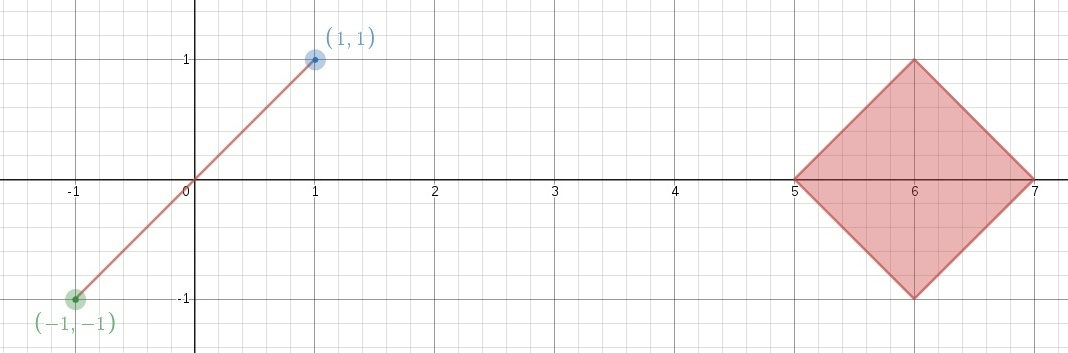
\includegraphics[width=\linewidth]{hw1-1.jpg}
\end{figure}\\
\begin{equation*}
\begin{aligned}
r_a = \sqrt{35}\\
r_b = \sqrt{35}\\
\rho(A, B) = \sqrt{35}\\
\end{aligned}
\end{equation*}
\section{} % 3
Найдем преобразование вида:
\begin{equation*}
f({\overline{x}})=\begin{pmatrix}
a & b\\
c & d
\end{pmatrix}{\overline{x}} +
\begin{pmatrix}
e\\
f
\end{pmatrix}
\end{equation*}
Преобразование изменяет точки: $A(0,0)\rightarrow P(3,6)$, $B(1,0)\rightarrow Q(1,-4)$,
$C(1,1) \rightarrow R(-3,-3)$, $D(0,1)\rightarrow S(-1,7)$. То есть:\\
\begin{equation*}
\begin{pmatrix}
a & b\\
c & d
\end{pmatrix}A +
\begin{pmatrix}
e\\
f
\end{pmatrix} = P
\end{equation*}
\begin{equation*}
\begin{pmatrix}
a & b\\
c & d
\end{pmatrix}B +
\begin{pmatrix}
e\\
f
\end{pmatrix} = Q
\end{equation*}
\begin{equation*}
\begin{pmatrix}
a & b\\
c & d
\end{pmatrix}C +
\begin{pmatrix}
e\\
f
\end{pmatrix} = R
\end{equation*}
\begin{equation*}
\begin{pmatrix}
a & b\\
c & d
\end{pmatrix}D +
\begin{pmatrix}
e\\
f
\end{pmatrix} = S
\end{equation*}
Получим две системы уравнений:
\begin{equation*}
  \begin{cases}
  aA_1 + bA_2 + e = P_1\\
  aB_1 + bB_2 + e = Q_1\\
  aC_1 + bC_2 + e = R_1\\
  aD_1 + bD_2 + e = S_1
  \end{cases}
  \;
  \begin{cases}
  cA_1 + dA_2 + f = P_2\\
  cB_1 + dB_2 + f = Q_2\\
  cC_1 + dC_2 + f = R_2\\
  cD_1 + dD_2 + f = S_2
  \end{cases}
\end{equation*}
Решение: $e=3$, $f=64$, $a= -2$, $b=-4$, $c=-10$, $d=1$.\\
Искомое преобразование:\\
\begin{equation*}
f({\overline{x}})=\begin{pmatrix}
-2 & -4\\
-10 & 1
\end{pmatrix}{\overline{x}} +
\begin{pmatrix}
3\\
6
\end{pmatrix}
\end{equation*}
%
\section{} % 4
%
$f({\overline{x}})= \left(
\begin{matrix}
\cos{\varphi} & -\sin{\varphi}\\
\sin{\varphi} & \cos{\varphi}\\
\end{matrix}
\right
)
\left ( {\overline{x}} -
\left(
\begin{matrix}
a_1\\
a_2\\
\end{matrix}
\right
)
\right ) \, +
\left(
\begin{matrix}
a_1\\
a_2\\
\end{matrix}
\right
)
$\\
\\
$\varphi = -\frac{2\pi}{3}$\\
$A=( \, -3, 4) \,$\\
\\
\begin{equation*} f({\overline{x}})= \frac{1}{2}\left(
\begin{matrix}
-1 & \sqrt{3}\\
-\sqrt{3} & -1\\
\end{matrix}
\right
)
\left ( {\overline{x}} -
\left(
\begin{matrix}
-3\\
4\\
\end{matrix}
\right
)
\right ) \, +
\left(
\begin{matrix}
-3\\
4\\
\end{matrix}
\right
)
\end{equation*}\\
\begin{equation*}
f({\overline{x}})= \frac{1}{2}\left(
\begin{matrix}
-1 & \sqrt{3}\\
-\sqrt{3} & -1\\
\end{matrix}
\right
)
{\overline{x}} + \frac{1}{2}
\left(
\begin{matrix}
-9 - 4\sqrt{3}\\
12 - 3\sqrt{3}\\
\end{matrix}
\right
)
\end{equation*}
\section{} % 5
\begin{figure}[h!]
  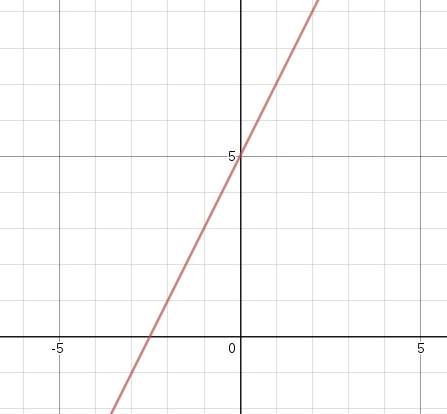
\includegraphics[width=\linewidth]{hw1-2.jpg}
\end{figure}
$x_2 = 2x_1 + 5$\\
$f({\overline{x}})= \left(
\begin{matrix}
\cos{2\Theta} & \sin{2\Theta}\\
\sin{2\Theta} & -\cos{2\Theta}\\
\end{matrix}
\right
)
\left ( {\overline{x}} -
\left(
\begin{matrix}
0\\
c\\
\end{matrix}
\right
)
\right ) \, +
\left(
\begin{matrix}
0\\
c\\
\end{matrix}
\right
)
$\\
\\
$\tan{\Theta} = 2\;\\  c = 5$\\
$\sin{2\Theta} = \frac{2\tan{\Theta}}{1+\tan^2{\Theta}}=\frac{4}{5}$\\
$\cos{2\Theta} = \frac{1-\tan^2{\Theta}}{1 + \tan^2{\Theta}} = - \frac{3}{5}$\\
\begin{equation*}
f({\overline{x}})= \frac{1}{5}\left(
\begin{matrix}
-3 & 4\\
4 & 3\\
\end{matrix}
\right
)
\left ( {\overline{x}} -
\left(
\begin{matrix}
0\\
5\\
\end{matrix}
\right
)
\right ) \, +
\left(
\begin{matrix}
0\\
5\\
\end{matrix}
\right
)\\
\end{equation*}
\begin{equation*}
f({\overline{x}})= \frac{1}{5}\left(
\begin{matrix}
-3 & 4\\
4 & 3\\
\end{matrix} \right )
{\overline{x}} +
\left(
\begin{matrix}
-4\\
2\\
\end{matrix}
\right
)
\end{equation*}
\end{document}
